\section{Experiments}
\label{sec:exp}
In this section, we first describe the dataset used in our paper. We then introduce all baselines and evaluation metric. Finally, we present our research questions and results.

\subsection{Dataset}
\label{sec:dataset}
\cmt{TODO: add the information about the dataset}

\subsection{Baseline}
\label{sec:baseline}
We compared DeepJIT with two other state-of-the-art baselines in the \emph{Just-In-Time} (JIT) defect prediction:
\begin{itemize}
\item JIT: The method for identifying fix-inducing code changes was proposed by McIntosh and Kamei~\cite{mcintosh2018fix}. The method used a nonlinear variant of multiple regression modeling~\cite{fox1997applied} to build a classification model for automatically identifying defects in commits. The set of code features, using six families of code change properties, were primarily derived from prior studies~\cite{Kamei:2013:LES, Kim:2008:CSC, Kononenko:2015, Mockus2000}. These properties were: the magnitude of change, the dispersion of the changes, the defect proneness of prior changes, the experience of the author, the code reviewers, and the degree of participation in the code review. 
\item DBN-JIT: The model adopted Deep Belief Network (DBN)~\cite{hinton2006reducing}, one of the state-of-the-art deep learning approaches in performing nonlinear dimensionality reduction, to generate a more expressive feature set from the initial feature set~\cite{Yang:2015:DLJ}. The generated feature set, a complicated nonlinear combination of the initial features, was put to a machine learning classifier~\cite{nasrabadi2007pattern} to predict defects in commits. 
\end{itemize}

\subsection{Training and hyperparameters}
\label{sec:training_parameters}
For the size of the convolutional filters, we choose 64. The size of DeepJIT's fully-connected layer described in Section~\ref{sec:ftr_combine} is set to 512. The word vectors dimension of the commit message ($d_m$) and code changes ($d_c$) are set to 64. We train DeepJIT using Adam~\cite{kingma2014adam} with shuffled mini-batches.  The batch size is set to 32. We train DeepJIT for 100 epochs. We also apply the early stopping strategy~\cite{prechelt1998automatic, caruana2001overfitting} to avoid overfitting problem during the training process. Typically, we stop the training if the value of the objective function (see Equation~\ref{eq:cost}) has been no update in the last 5 epochs. All these hyperparameters in our paper are widely used in the deep learning community~\cite{severyn2015learning, huo2016learning, huo2017enhancing, hinton2012improving}. 
 
\subsection{Evaluation Metric}
\label{sec:metric}
To evaluate the accuracy of \emph{Just-In-Time} (JIT) models, we calculate  threshold-independent measures of model performance. Since our dataset is imbalanced data, we avoid using threshold-dependent measures (i.e., precision, recall, or F1) since these measures strongly depend on arbitraily thresholds~\cite{nguyen2009learning, gu2008data}. Following the previous work~\cite{mcintosh2018fix},  we use the Area Under the receiver operator characteristics
Curve (AUC) to measure the power of models' discriminatory, i.e., their ability to differentiate between defects or clean commits. AUC computes the area under the curve plotting the true positive rate against the false positive rate, while applying multiple thresholds to determine if a commit is buggy or not. The values of AUC normally are ranged between 0 (worst discrimination) and 1 (perfect discrimination). 

\subsection{Research Questions and Results}
\label{sec:rq_results}

\noindent \textbf{RQ1: How effective is DeepJIT compared to the state-of-the-art baseline?}

\begin{figure}
	\center
	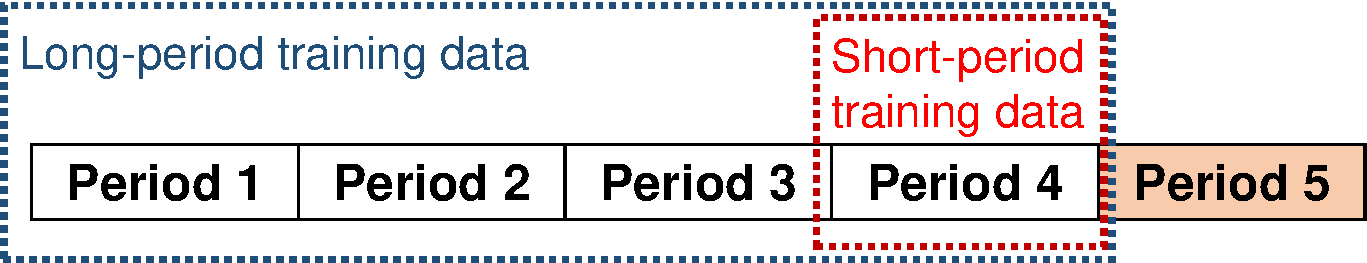
\includegraphics[scale=0.36]{figs/split.pdf}
	\caption{An example of choosing the training data for short-period and long-period models. The last period will be used as testing data.}
	\label{fig:splitting}
\end{figure}

To address RQ1, we evaluate how a JIT model, which is trained by a train data, can be used to predict a test data. Typically, we train three types of JIT models: 
\begin{itemize}
\item \textbf{Random models:} To evaluate machine learning algorithm, most people use $k$-fold cross-validation~\cite{kohavi1995study} in which a dataset is randomly divided to $k$ folds, each fold is considered as test data for evaluating JIT model while $k - 1$ folds are considered as train data. In this case, the JIT model is trained on a mixture of past and future data. In our paper, we set $k = 5$.
\item \textbf{Short-period models:} The JIT model is trained using commits that occurred at one time period. We assume that older commits changes may have characteristics that no longer effects to the latest commits. 
\item \textbf{Long-period models:} Inspired by the work~\cite{rahman2013sample}, suggesting that larger amounts of training data tend to achieve a better performance in defect prediction problem, we train the JIT model using all commits that occurred before a particular period. We discover whether additional data may improve the performance of the JIT model. 
\end{itemize} 

Figure~\ref{fig:splitting} describes how the training data is selected to train short-period and long-period models. We use the last period (i.e., period 5) as a testing data. While the short-period model is trained using the commits that occurred during period 4, the long-period model is trained using the commits that occurred from period 1 to period 4. After training the short-period and long-period model, we measure their performance of these models using AUC described in Section~\ref{sec:metric}.

Table~\ref{tab:results} shows the AUC results of DeepJIT as well as other baselines in three types of JIT models setting: random, short-period, and long-period. The difference between random models compared to short-period and long-period models is quite small (i.e., below 2.2\%) which suggests that there is no difference between training on past or future data. \cmt{TODO: Prof. Hoa, do you have any explaination about it?} In the QT project, DeepJIT achieves AUC scores of 0.768, 0.764, and 0.765 in three different JIT settings: random, short-period, and long-period, respectively. Comparing them to the best performing baseline (i.e., DBNJIT), DeepJIT constitute improvements of 8.96\%, 7.00\%, and 8.05\% in term of AUC. In the OPENSTACK project, DeepJIT also constitute improvements of 8.21\%, 9.08\%, and 8.29\% in term of AUC compared to DBNJIT (the best performing baseline). 

%To evaluate machine learning algorithm, most people use $k$-fold cross-validation~\cite{kohavi1995study} in which a dataset is randomly divided to $k$ folds, each fold is 
%
%A common strategy for evaluating machine learning
%algorithms is $n$-fold cross-validation~\cite{kohavi1995study},
%in which a dataset is randomly distributed among $n$ equal-sized buckets,
%each of
%which is considered as test data for a model trained on the contents of the
%remaining $n-1$ buckets.  When data elements become available over time, as
%is the case of Linux kernel patches, this strategy can result in testing a
%model on data that predates some of the data on which the model was
%trained.  Respecting the order in which patches are submitted,
%however, would limit the amount of testing that can be done, given
%the fairly small number of stable patches available.
%
%To address this issue, we first assess whether training on future data
%helps or harms the accuracy of PatchNet on our dataset.  We first sort the
%patches collected in Section~\ref{sec:data} from earliest to latest based
%on the date when the patch author submitted the patch to maintainers. Then,
%we divide the dataset into 5 mutually exclusive sets by date. Note that the
%resulting five sets are not perfectly balanced, but they come close, with
%stable patches making up 45\% to 55\% of each set.  Then, we repeat the
%following process five times: take one set as a testing set and use the
%remaining four sets for training. When we test on the first set, we observe
%the impact of training only on future data.  When we test on the fifth set,
%we observe the impact of training only on past data.  The other testing
%sets use models trained on a mixture of past and future data.
%
%Table~\ref{tab:cross_valid_patchnet} shows the results of PatchNet on the
%different test sets. The standard deviations are quite small (i.e., below
%0.013), hence there is no difference between training on past or future
%data.  Our dataset starts with Linux v3.0, which was released in 2011,
%twenty years after the start of work on the Linux kernel.  The lack of
%impact due to training on past or future data suggests that in such a
%mature code base the properties that make a patch relevant for stable
%kernels are fairly constant over time.  This property is indeed beneficial,
%because it means that our approach can be used to identify stable-relevant commits that have been missed in older versions.  In subsequent research
%questions, we thus retain the same five test and training sets.


\begin{table*}[t!]
	\centering
	\caption{The AUC results of DeepJIT vs. with other baselines in three types of JIT models: random, short-period, and long-period.}
	\begin{tabular}{|l|c|c|c|c|c|c|}
		\hline
		\multirow{2}[4]{*}{} & \multicolumn{3}{c|}{QT} & \multicolumn{3}{c|}{OPENSTACK} \\
		\cline{2-7}          & Random & Short-Period & Long-period & Random & Short-Period & Long-period \\
		\hline
		\hline
		JIT   & 0.701 & 0.703 & 0.702 & 0.691 & 0.711 & 0.706 \\
		\hline
		DBNJIT & 0.705 & 0.714 & 0.708 & 0.694 & 0.716 & 0.712 \\
		\hline
		DeepJIT & \textbf{0.768} & \textbf{0.764} & \textbf{0.765} & \textbf{0.751} & \textbf{0.781} & \textbf{0.771} \\
		\hline
	\end{tabular}%
	\label{tab:results}%
\end{table*}%

\noindent \textbf{RQ2: Does the proposed model benefit both commit message and the code changes?}

To answer this question, we employ an ablation test~\cite{korbar2017deep, liu2017deep}, by ignoring the commit message and the code change in a commit and then evaluate the AUC performance. Specifically, we create two different variants of DeepJIT, namely DeepJIT-Msg and DeeJIT-Code. DeepJIT-Msg only considers commit message information while DeepJIT-Code only uses commit code information. We again use the three types of model settings (i.e., random, short-period, and long period) to evaluate the AUC score. 


%o  answer  this  RQ,  we  conduct  an  ablation  test  [33],[42]  by  ignoring  the  commit  message,  the  code  changes,or  the  function  names  in  the  code  changes  in  a  givenpatch  one-at-a-time  and  evaluating  the  performance.  Wecreate  three  variants  of  PatchNet:  PatchNet-C,  PatchNet-M,  and  PatchNet-NN.  PatchNet-C  uses  only  code  changeinformation  while  PatchNet-M  uses  only  commit  messageinformation. PatchNet-NN uses both code change and com-
%mit message information, but ignores the function names inthe code changes. We again use the five copies of the datasetdescribed in RQ1 and compute the various evaluation met-rics.Table  3  shows  that  the  performance  of  PatchNet  de-grades if we ignore any one of the considered types of in-formation. Accuracy, precision, recall, F1, and AUC drop by19.39%, 15.41%, 21.26%, 18.34%, and 16.06% respectively ifwe ignore commit messages. They drop by 16.96%, 14.62%,16.58%, 14.76%, and 14.21% respectively if we ignore codechanges. And they drop by 11.08%, 12.62%, 16.43%, 13.86%,and 11.98% respectively if we ignore function names. Thus,each  kind  of  information  contributes  to  PatchNet’s  perfor-mance.  Additionally,  the  drops  are  greatest  if  we  ignorecommit  messages,  indicating  that  they  are  slightly  moreimportant than the other two to PatchNet’s performance

\begin{table*}[t!]
  \centering
  \caption{Contribution of feature components in DeepJIT}
    \begin{tabular}{|l|c|c|c|c|c|c|}
    \hline
    \multirow{2}[4]{*}{} & \multicolumn{3}{c|}{QT} & \multicolumn{3}{c|}{OPENSTACK} \\
\cline{2-7}          & \multicolumn{1}{l|}{Short-Period} & \multicolumn{1}{l|}{Long-period} & \multicolumn{1}{l|}{Random} & \multicolumn{1}{l|}{Short-Period} & \multicolumn{1}{l|}{Long-period} & \multicolumn{1}{l|}{Random} \\
    \hline
    \hline
    DeepJIT-Msg & 0.609 & 0.638 & 0.641 & 0.583 & 0.659 & 0.689 \\
    \hline
    DeepJIT-Code & 0.734 & 0.727 & 0.738 & 0.769 & 0.738 & 0.729 \\
    \hline
    DeepJIT & \textbf{0.764} & \textbf{0.765} & \textbf{0.768} & \textbf{0.781} & \textbf{0.771} \\
    \hline
    \end{tabular}%
  \label{tab:variants}%
\end{table*}%

\noindent \textbf{RQ3: Does the proposed model benefit from the manually extracted code changes features?}

\begin{table*}[t!]
  \centering
  \caption{Combination of DeepJIT with JIT's features}
    \begin{tabular}{|l|c|c|c|c|c|c|}
    \hline
    \multirow{2}[4]{*}{} & \multicolumn{3}{c|}{QT} & \multicolumn{3}{c|}{OPENSTACK} \\
\cline{2-7}          & Short-Period & Long-period & Random & Short-Period & Long-period & Random \\
    \hline
    \hline
    DeepJIT & 0.764 & 0.765 & 0.768 & 0.781 & 0.771 & 0.751 \\
    \hline
    DeepJIT-Combined & \textbf{0.788} & \textbf{0.786} & \textbf{0.779} & \textbf{0.814} & \textbf{0.799} & \text{0.760} \\
    \hline
    \end{tabular}%
  \label{tab:combined}%
\end{table*}%

\noindent \textbf{RQ4: How are the time costs of the proposed model?}


